\section{基本几何体}

根据表面形状的不同可以将基本几何体分为平面立体和曲面立体。如果立体表面均由平面构成,则称为平面立体,如长方体、正方体、棱柱、棱锥、棱台等。如果立体表面由平面和曲面共同构成或全部由曲面构成,则称为曲面立体,如圆柱、圆球、圆环等。
\subsection{平面立体}

\subsubsection{棱柱体}



图\ref{fig:sannenzhu}所示的正三棱柱,其顶面与底面的水平面投影重合并反映实形,为一正三角形。三个棱面在水平投影面积聚为三角形的三条边。三棱柱的三视图投影如图\ref{fig:sannenzhuthreeview}所示。
\begin{figure}[htbp]
\centering
\subfloat[]{\label{fig:sannenzhu}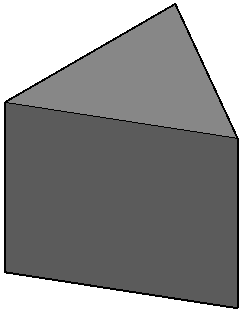
\includegraphics[scale=0.6]{sannenzhu.png}}\hspace{30pt}
\subfloat[]{\label{fig:sannenzhuthreeview}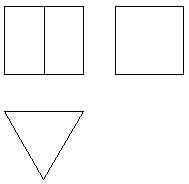
\includegraphics[scale=1]{sannenzhuthreeview.png}}
\caption{正三棱柱的投影}
\end{figure}



由此可见棱柱体的投影特点是:一面投影反映底面实形,其余两面投影则为矩形或复合矩形。
\subsubsection{棱锥体}
棱锥体是由一个多边形底面和若干个共顶点的三角形棱面构成的。从棱锥体顶点到底面的垂直距离称为棱锥体的高。如果棱锥体的底面为正多边形,锥顶的投影位于多边形的中心,各棱面是等腰三角形,则该棱锥体称为正棱锥。正四棱锥的三面投影如图\ref{fig:fournenzhuithreeview}所示。

\begin{figure}[htbp]
\centering
\subfloat[]{\label{fig:fournengzhui}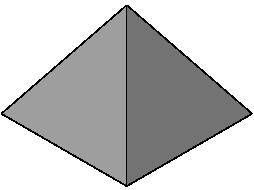
\includegraphics[scale=0.9]{fournengzhui.png}}\hspace{30pt}
\subfloat[]{\label{fig:fournenzhuithreeview}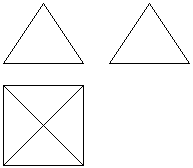
\includegraphics[scale=1]{fournenzhuithreeview.png}}
\caption{正四棱锥的投影}
\end{figure}

图\ref{fig:fournengzhui}所示的正四棱锥的底面与水平投影面平行,其投影反映实形,为正方形;底面在其它投影面积聚为一条直线;棱面的三面投影则为类似的三角形。

由此可见,棱锥体的投影特点是:一投影面为由三角形构成的复合多边形,其两投影为三角形或复合三角形。
\subsubsection{棱台体}
棱台体是由棱锥体被切掉顶部后所构成的一种形体。棱台体的投影特点是:一面投影为由梯形构成的内外相似复合多边形,其余两面投影则为梯形或复合梯形。图\ref{fig:fivenentai} 所示为五棱台的投影。
\begin{figure}[htbp]
\centering
\subfloat[]{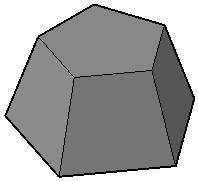
\includegraphics[scale=0.9]{fivenentai.png}}\hspace{30pt}
\subfloat[]{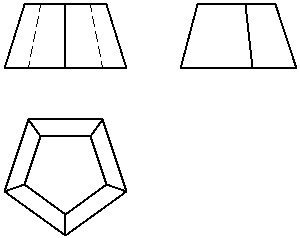
\includegraphics[scale=1]{fivenentaithreeview.png}}
\caption{五棱台的投影}\label{fig:fivenentai}
\end{figure}

\subsection{曲面立体}
曲面体是由面或曲面和平面共同构成的立体,其中最常见的是回转曲面。回转体曲面是

\subsubsection{圆柱体}
圆柱体是由圆柱面、顶面、底面所构成的。圆柱体可以看作一条与轴线平行的母线绕轴线旋转而成的。图\ref{fig:yuanzhutix}所示圆柱体的轴线垂直于水平投影面,其水平投影为圆;其正投影和侧投影均为矩形。
\begin{figure}[htbp]
\centering
\subfloat[]{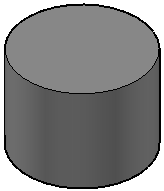
\includegraphics[scale=0.9]{yuanzhuti.png}}\hspace{30pt}
\subfloat[]{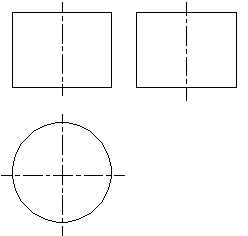
\includegraphics[scale=0.7]{yuanzhutithreeview.png}}
\caption{圆柱体的投影}\label{fig:yuanzhutix}
\end{figure}

\subsubsection{球体}
球体是由圆形母线以其直径为回转轴旋转而成的。球体的三面投影均为圆。

\begin{figure}[tbp]
\centering
\subfloat[]{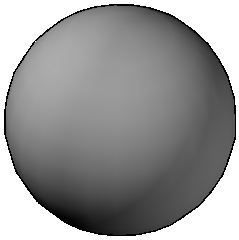
\includegraphics[scale=0.7]{qiouti.png}}\hspace{30pt}
\subfloat[]{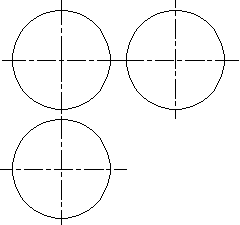
\includegraphics[scale=0.7]{qioutithreeview.png}}
\caption{球体的投影}\label{fig:qiout}
\end{figure}

\endinput